\chapter{Additional material on \ssww prospects at the HL-LHC}\label{app:sswwupgrade_additional_material}

\section{Truth isolation}\label{app:truth_isolation}
As mentioned in Section~\ref{sswwupgrade:isolation}, the size of the background contribution from top processes are much larger than expected when no isolation is applied.
The event yields using an earlier version of the event selection with no truth-based isolation requirement are listed in Table~\ref{tab:truth_iso_noiso}.
Here, top events make up nearly 90\% of the total background, and the contributions from fake and charge-flipped electrons are also large.
The event yields using the same event selection with the truth-based isolation included are shown in Figure~\ref{tab:truth_iso_tightiso}.
When comparing the two tables, the considerable reduction in the top background can be clearly seen.
\begin{table}[htp]
  \centering
  \begin{tabular}{l|rrrrr}
    yields by type&all channels&$\mu\mu$&$ee$&$\mu e$&$e\mu$\\
    \hline\hline
    signal&4011&1583.2&531.7&793.1&1103.1\\
    ww qcd&252.6&105.8&30.4&48&68.4\\
    charge flip&2528.4&0.0&2075.4&255.1&197.8\\
    fakes&7135.4&0.0&4675.1&1904.3&555.9\\
    diboson&2370.4&581.2&491.8&517.9&779.6\\
    triboson&125.5&49.1&17.8&24.6&34.1\\
    top&90150.5&26618&15301.6&25277.9&22953.1\\
    z+jets&241.2&0.0&0.0&0.0&241.2\\
    w+jets&31.4&3.9&7.6&13.2&6.7\\
    \hline
    total bkg&102803.9&27354&22592&28027.8&24830.1\\
    signal&4011&1583.2&531.7&793.1&1103.1\\
    \hline
  \end{tabular}
  \caption{Event yields prior to applying any form of truth-based isolation criteria.}
  \label{tab:truth_iso_noiso}
\end{table}


\begin{table}[htp]
  \centering
  \begin{tabular}{l|rrrrr}
    yields by type&all channels&$\mu\mu$&$ee$&$\mu e$&$e\mu$\\
    \hline\hline
    signal&3470.5&1427.3&428.8&675.8&938.7\\
    ww qcd&205.8&90.8&22.7&38.3&54\\
    charge flip&2398.3&0.0&2104.6&95.8&197.9\\
    fakes&4309.7&0.0&3390.6&750.8&168.3\\
    diboson&1552.4&311.3&355.6&346.8&538.7\\
    triboson&115&46.8&15.4&21.6&31.2\\
    top&156.9&42.3&14.8&76.6&23.3\\
    z+jets&0.0&0.0&0.0&0.0&0.0\\
    w+jets&0.3&0.0&0.0&0.3&0.0\\
    \hline
    total bkg&8738.1&491.3&5903.7&1329.8&1013.4\\
    signal&3470.5&1427.3&428.8&675.8&938.7\\
    \hline
  \end{tabular}
  \caption{Event yields after applying a test version of the truth-based isolation.}
  \label{tab:truth_iso_tightiso}
\end{table}


\TODO{Add tables for tight vs loose working point, information on the necessity of TRUTH1++}
\FloatBarrier

\subsection{\tt{TRUTH1++} derivations}
The ATLAS standard \tt{TRUTH1} derivations used for this analysis contain a slimmed truth particle container in order to reduce the file size.
As a result, many of the truth particles that would be included in the isolation variables are missing, and the truth-based isolation will not accurately model the reconstruction-level isolation variables.
In order to recover the performance of the truth-based isolation in the top MC samples (where it is most needed), a custom derivation was produced privately that duplicated the default \tt{TRUTH1} data structure but includes the full truth particle record.
The reduced size of the truth particle information in the \tt{TRUTH1} derivation compared to the \tt{TRUTH1++} derivation is shown in Figure~\ref{fig:truth_iso_truth1}.

\begin{figure}[htbp]
  \centering
  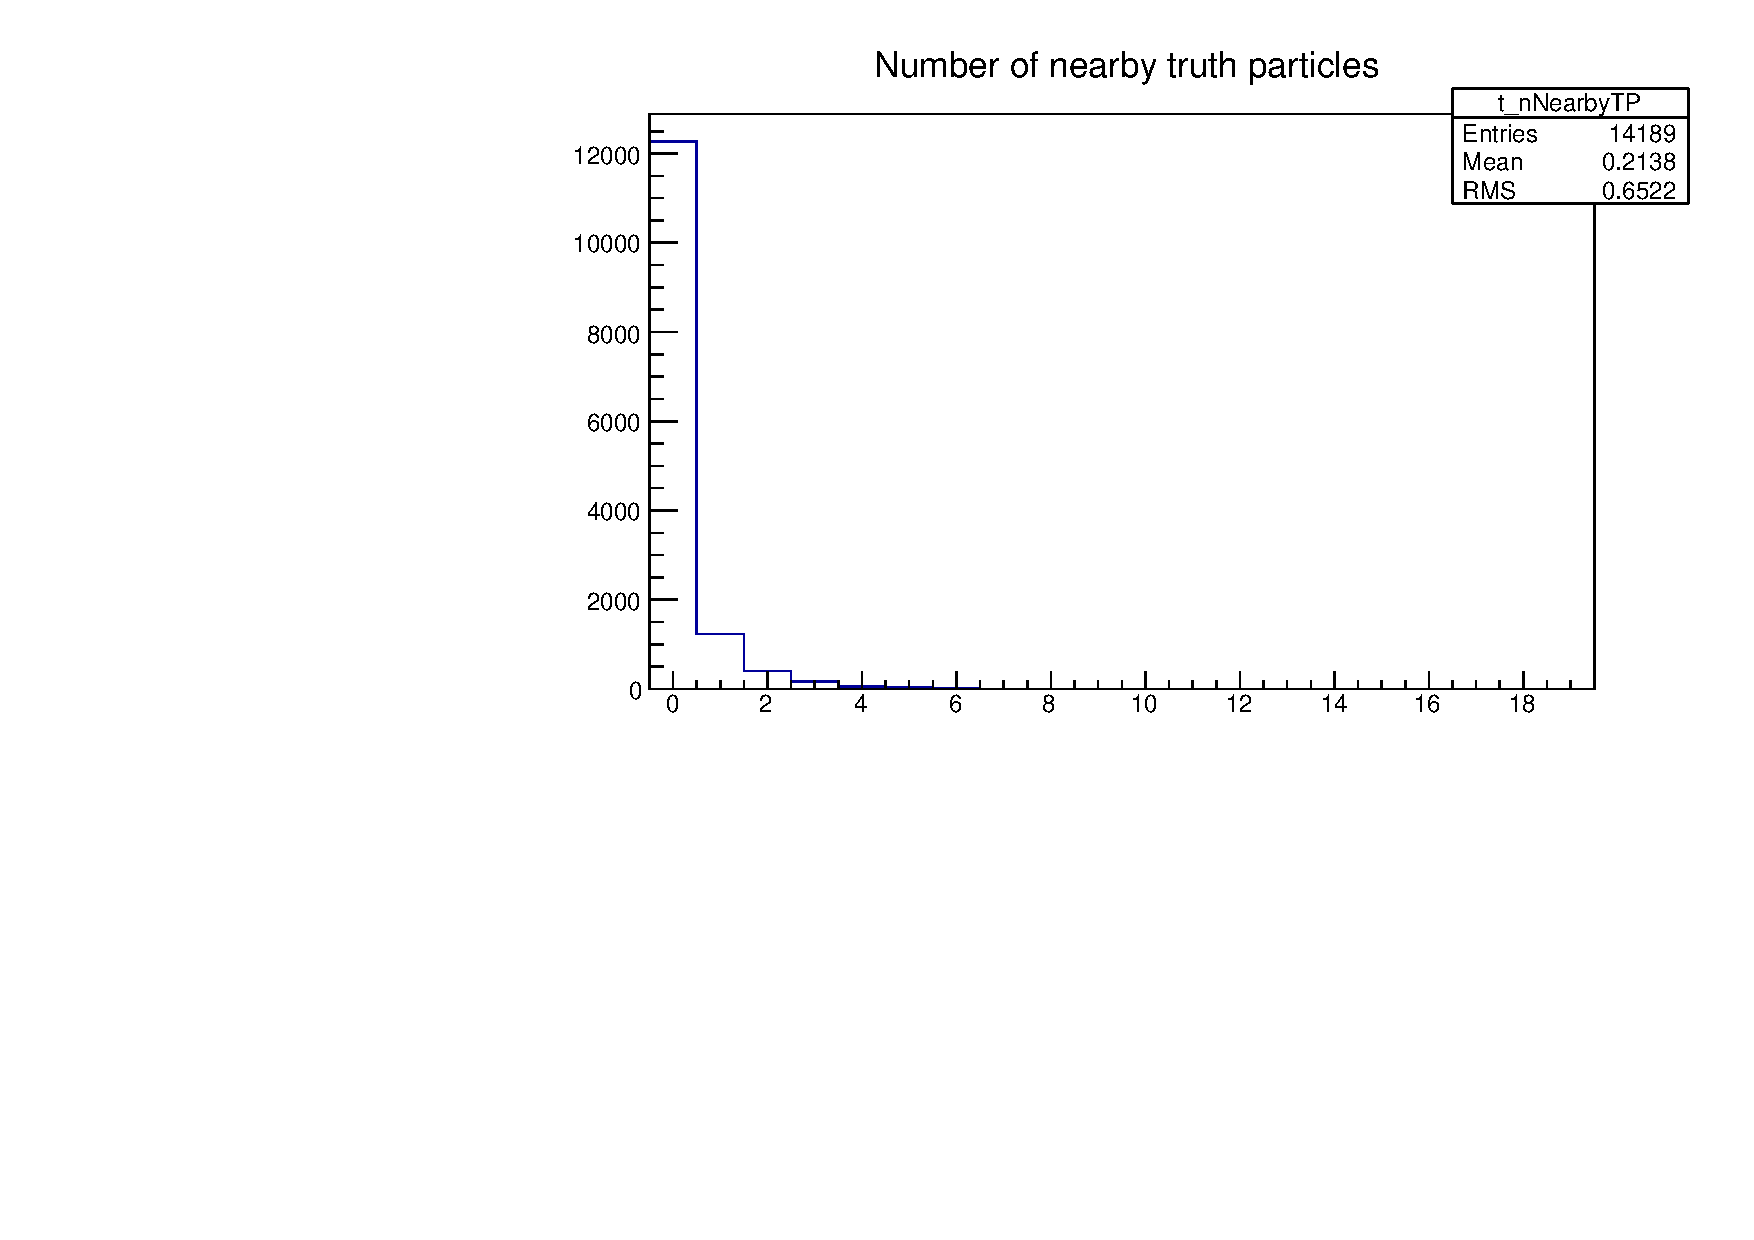
\includegraphics[width=.48\textwidth]{figs/ssww_upgrade/isolation/truth1_nearbytp}
  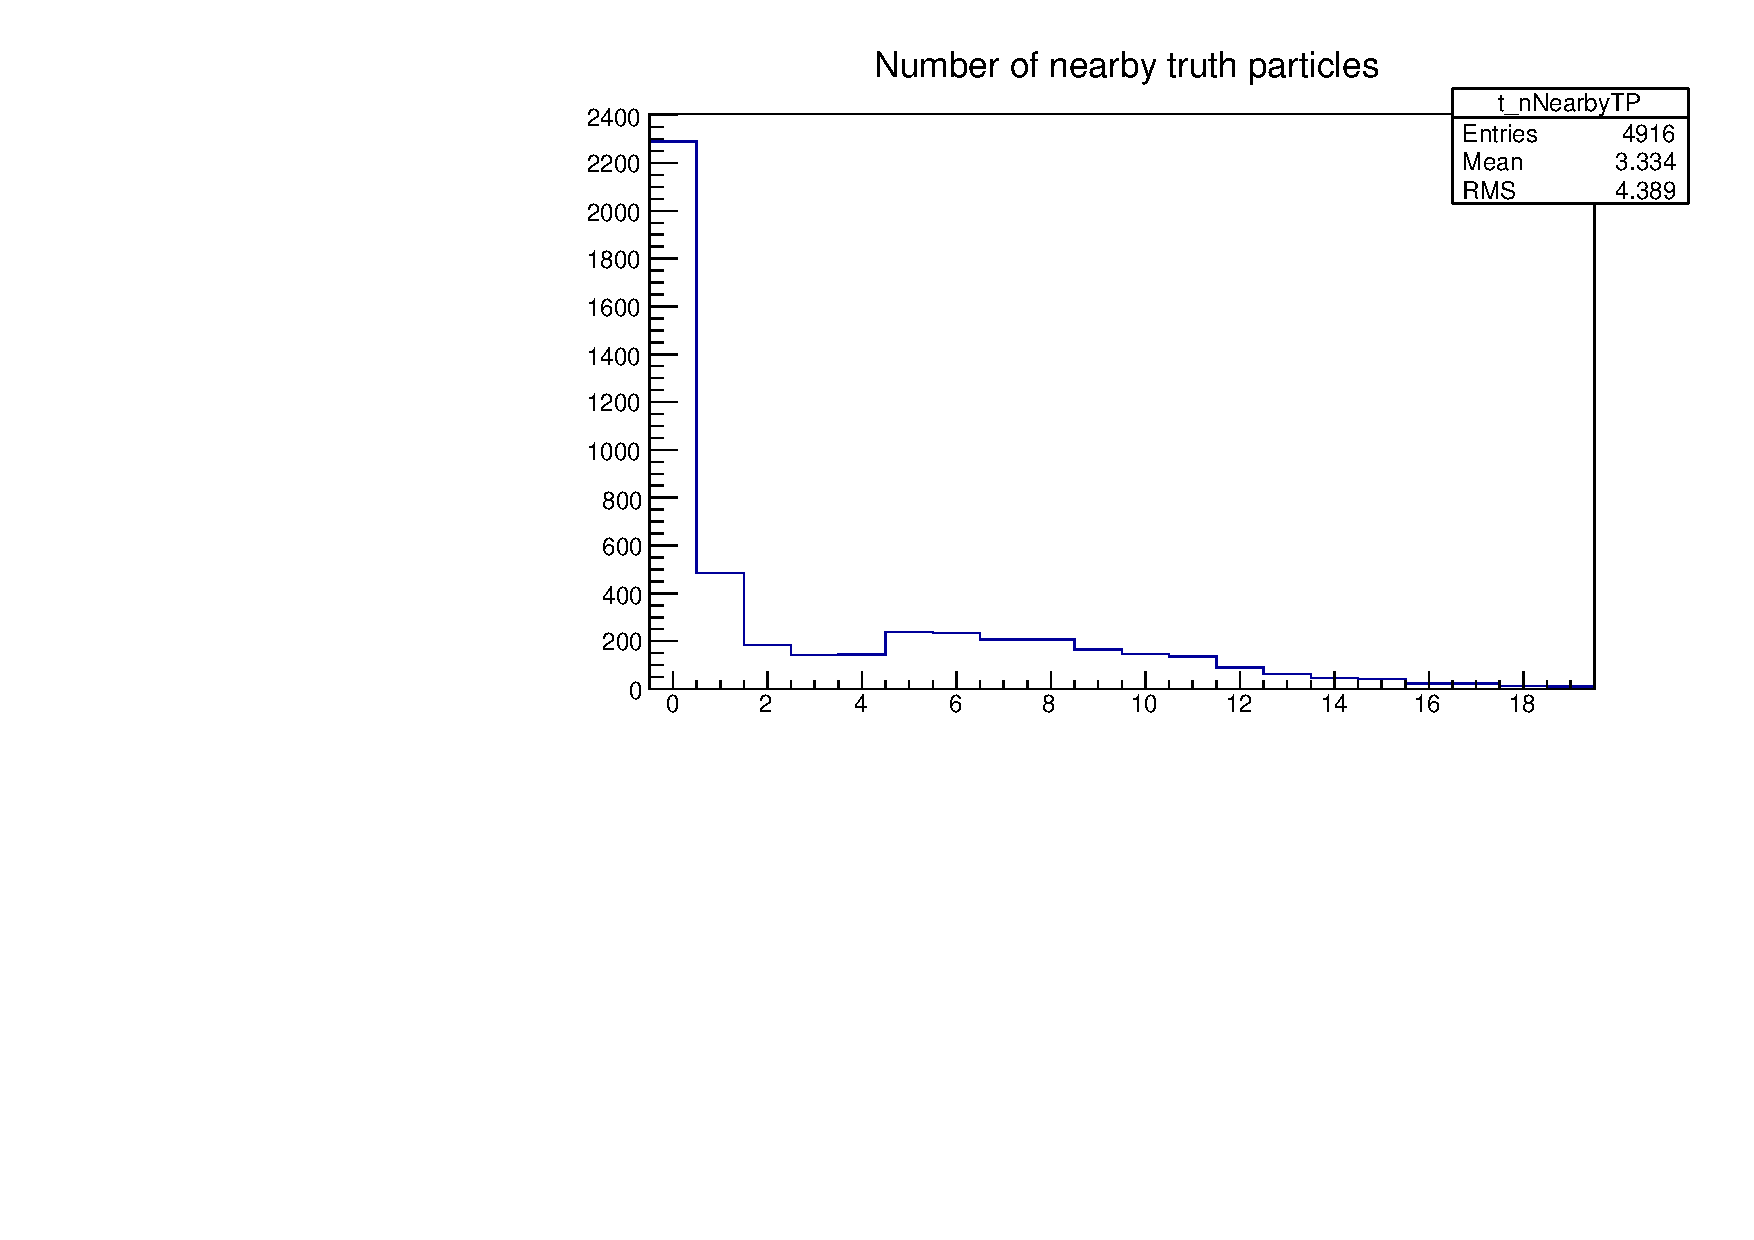
\includegraphics[width=.48\textwidth]{figs/ssww_upgrade/isolation/truth1pp_nearbytp}
  \caption{Number of truth particles within $\deltar < 0.4$ of a selected muon or electron using the ATLAS standard \tt{TRUTH1} (left) and the custom \tt{TRUTH1++} (right) derivations in $t\bar{t}$ simulation. The complete truth record is stored in the \tt{TRUTH1++} derivation, and this is best seen in the first bin, where the lepton has no nearby truth particles.}
  \label{fig:truth_iso_truth1}
\end{figure}
\FloatBarrier

\subsection{Check of truth-based isolation}
Since the isolation variables are constructed from truth particles, there is an expectation that the efficiency of the isolation selection will be higher than what would be seen in the full simulation.
In order to test this, a truth-level $13\tev$ $t\bar{t}$ MC sample was run through a selection altered to mimic the 13~TeV \ssww measurement as closely as possible.
The results were compared to the $t\bar{t}$ background in the $13\tev$ analysis extrapolated to $14\tev$ and $3000~\textrm{fb}^{-1}$, and the truth-based isolation reduces the expected events by a factor of approximately 4.
However, the statistics in the $13\tev$ truth-level sample are low, and it is therefore difficult to measure precisely how much the truth-based isolation overperforms.

\subsection{Loose isolation working point}
As another check on the truth-based isolation, a second isolation working point was constructed to match the official ATLAS Fixed Cut Loose isolation working point.
The definition of this loose isolation are found in Table~\ref{tab:isolation_cuts_loose}.

The primary impact of loosening the isolation is a substantial increase in the non-prompt background from top processes, and a moderate increase in the charge mis-ID and fake backgrounds.
Backgrounds from prompt leptons only did not see major changes.
As a result, the tight working point is chosen for the analysis.
The event yields by sample and by background type using the loose working point are in Table~\ref{tab:EY_loose}, and Table~\ref{tab:EY_tight} has the numbers using the tight working point (defined in Table~\ref{tab:truth_iso_definition}) for comparison.

\begin{table}[htbp]\renewcommand{\arraystretch}{1.2}
  \begin{center}
 % \scalebox{0.75}{
  \begin{tabular}{l|c|c}
    \hline\hline
				~               &   Electron Isolation & Muon Isolation \\
\hline\hline
Track-based isolation cone size   		&   $\deltar < 0.2$         & $\deltar < 0.3$ \\
Track-based isolation requirement    		&   $\sum\pt/\pt^{e} < 0.15$ & $\sum\pt/\pt^{\mu} < 0.15$ \\
Calorimeter-based isolation cone size   	&   $\deltar < 0.2$	    & $\deltar < 0.2$\\
Calorimeter-based isolation requirement    	&   $\sum\et/\pt^{e} <  0.2$ & $\sum\et/\pt^{\mu} <  0.3$	\\
\hline
 \end{tabular}
  %}
  \end{center}
  \caption{Electron and muon isolation requirements for the loose working point.} 
  \label{tab:isolation_cuts_loose}
\end{table}

\begin{sidewaystable}[!htbp]
  {\scriptsize
    \begin{tabular}{r|rrr|rrr|rrr|rrr|rrr}
      run number&\multicolumn{3}{c|}{all channels}&\multicolumn{3}{c|}{mm}&\multicolumn{3}{c|}{ee}&\multicolumn{3}{c|}{me}&\multicolumn{3}{c}{em}\\
      \hline
      &events&stat&sys&events&stat&sys&events&stat&sys&events&stat&sys&events&stat&sys\\
      \hline\hline
      ssWW ewk&3783.20&22.08&0.00&1524.99&15.00&0.00&484.74&7.01&0.00&740.76&9.01&0.00&1032.72&11.50&0.00\\
      
      charge flip&3025.40&1276.74&0.00&0.00&0.00&0.00&2615.30&1267.89&0.00&197.20&87.94&0.00&212.90&121.63&0.00\\
      
      ssWW qcd&223.95&3.54&44.79&97.17&2.51&19.43&25.51&1.03&5.10&42.23&1.40&8.45&59.04&1.80&11.81\\
      
      fakes&5315.55&1775.87&0.00&0.00&0.00&0.00&3524.24&1694.39&0.00&1356.74&450.60&0.00&434.57&282.33&0.00\\
      
      363507&14.87&1.28&2.23&3.41&0.62&0.51&3.25&0.50&0.49&3.14&0.51&0.47&5.08&0.86&0.76\\
      
      363508&0.31&0.04&0.05&0.04&0.01&0.01&0.13&0.03&0.02&0.04&0.01&0.01&0.11&0.03&0.02\\
      
      363509&4.22&0.37&0.63&0.82&0.18&0.12&1.26&0.19&0.19&0.70&0.14&0.11&1.44&0.23&0.22\\
      
      363627&0.89&0.89&0.00&0.00&0.00&0.00&0.00&0.00&0.00&0.89&0.89&0.00&0.00&0.00&0.00\\
      
      363633&0.28&0.28&0.00&0.00&0.00&0.00&0.00&0.00&0.00&0.28&0.28&0.00&0.00&0.00&0.00\\
      
      363639&0.02&0.02&0.00&0.00&0.00&0.00&0.00&0.00&0.00&0.02&0.02&0.00&0.00&0.00&0.00\\
      
      363666&0.02&0.02&0.00&0.00&0.00&0.00&0.00&0.00&0.00&0.00&0.00&0.00&0.02&0.02&0.00\\
      
      363718&1739.72&34.34&173.97&446.19&18.22&44.62&354.25&17.12&35.43&378.06&14.37&37.81&561.22&18.65&56.12\\
      
      364242&7.74&1.12&1.16&2.56&0.70&0.38&0.80&0.32&0.12&1.56&0.45&0.23&2.81&0.69&0.42\\
      
      364243&2.39&0.46&0.36&0.61&0.25&0.09&0.58&0.23&0.09&0.50&0.19&0.08&0.70&0.25&0.10\\
      
      364245&0.27&0.05&0.04&0.06&0.02&0.01&0.08&0.03&0.01&0.02&0.01&0.00&0.11&0.03&0.02\\
      
      364246&0.74&0.15&0.11&0.12&0.07&0.02&0.16&0.07&0.02&0.20&0.08&0.03&0.27&0.10&0.04\\
      
      364250&53.73&14.51&5.37&4.72&2.46&0.47&12.65&6.17&1.27&2.48&1.25&0.25&33.89&12.84&3.39\\
      
      364255&8.13&4.72&0.81&0.00&0.00&0.00&0.00&0.00&0.00&5.15&3.66&0.52&2.98&2.98&0.30\\
      
      364284&394.02&6.26&39.40&97.81&2.37&9.78&84.37&1.79&8.44&84.92&5.02&8.49&126.92&2.27&12.69\\
      
      364336&44.93&2.48&6.74&19.68&1.77&2.95&4.55&0.66&0.68&8.58&0.96&1.29&12.13&1.29&1.82\\
      
      364337&27.71&1.96&4.16&12.36&1.30&1.85&2.75&0.51&0.41&5.22&0.96&0.78&7.38&0.97&1.11\\
      
      364338&7.61&3.17&1.14&5.77&2.89&0.87&0.96&0.96&0.14&0.88&0.88&0.13&0.00&0.00&0.00\\
      
      364339&6.62&3.39&0.99&2.12&2.12&0.32&1.31&1.31&0.20&1.27&1.27&0.19&1.91&1.91&0.29\\
      
      410155&74.78&11.74&11.22&30.97&8.27&4.65&16.51&4.04&2.48&10.08&4.82&1.51&17.22&5.47&2.58\\
      
      410218&18.56&3.94&2.78&0.00&0.00&0.00&6.27&2.26&0.94&1.71&1.51&0.26&10.58&2.85&1.59\\
      
      410219&6.68&2.85&1.00&3.78&2.45&0.57&0.00&0.00&0.00&1.48&0.92&0.22&1.42&1.12&0.21\\
      
      410220&9.46&2.83&1.42&3.26&1.83&0.49&0.44&1.04&0.07&3.06&1.24&0.46&2.70&1.44&0.40\\
      
      410501&289.04&152.68&43.36&191.25&135.24&28.69&37.93&37.93&5.69&59.85&59.85&8.98&0.00&0.00&0.00\\
      
      410642&156.12&156.12&23.42&0.00&0.00&0.00&0.00&0.00&0.00&156.12&156.12&23.42&0.00&0.00&0.00\\
      \hline\hline
      signal&3783.21&22.08&0.00&1524.99&15.00&0.00&484.74&7.01&0.00&740.76&9.01&0.00&1032.72&11.50&0.00\\
      
      ww qcd&223.95&3.54&44.79&97.17&2.51&19.43&25.51&1.03&5.10&42.23&1.40&8.45&59.04&1.80&11.81\\
      
      charge flip&3025.40&1276.74&0.00&0.00&0.00&0.00&2615.30&1267.89&0.00&197.20&87.94&0.00&212.90&121.63&0.00\\
      
      fakes&5315.55&1775.87&0.00&0.00&0.00&0.00&3524.24&1694.39&0.00&1356.74&450.60&0.00&434.57&282.33&0.00\\
      
      diboson&2195.61&38.10&219.58&548.72&18.54&54.87&451.27&18.29&45.14&470.61&15.71&47.07&725.01&22.95&72.50\\
      
      triboson&117.43&5.90&17.62&47.55&4.32&7.13&15.83&1.94&2.37&22.11&2.18&3.32&31.94&2.76&4.80\\
      
      top&554.63&218.75&83.21&229.26&135.53&34.40&61.15&38.23&9.18&232.30&167.28&34.85&31.92&6.43&4.78\\
      
      z+jets&0.00&0.00&0.00&0.00&0.00&0.00&0.00&0.00&0.00&0.00&0.00&0.00&0.00&0.00&0.00\\
      
      w+jets&1.21&0.87&0.00&0.00&0.00&0.00&0.00&0.00&0.00&1.19&0.87&0.00&0.02&0.00&0.00\\
      \hline
      total bkg&11433.78&2198.44&239.70&922.70&136.88&67.99&6693.30&2116.67&46.41&2322.38&488.89&59.27&1495.40&308.36&73.77\\
      
      signal&3783.21&22.08&0.00&1524.99&15.00&0.00&484.74&7.01&0.00&740.76&9.01&0.00&1032.72&11.50&0.00\\
      \hline\hline
    \end{tabular}
  }
  \caption{Event yields broken down by sample and by background type using the loose isolation workingpoint.  The sample ID's correspond to those listed in Table~\ref{tab:mc}; sample ID's between 363600 and 363671 correspond to the $W$+jets samples.  Events contining a fake or charge-flipped electron are removed from their respective sample and added to the ``fakes'' and ``charge flip'' rows, respectively.}
  \label{tab:EY_loose}
\end{sidewaystable}

\begin{sidewaystable}[!htbp]
  {\scriptsize
    \begin{tabular}{r|rrr|rrr|rrr|rrr|rrr}
      run number&\multicolumn{3}{c|}{all channels}&\multicolumn{3}{c|}{mm}&\multicolumn{3}{c|}{ee}&\multicolumn{3}{c|}{me}&\multicolumn{3}{c}{em}\\
      \hline
      &events&stat&sys&events&stat&sys&events&stat&sys&events&stat&sys&events&stat&sys\\
      \hline\hline
      signal&3489.49&21.23&0.00&1434.85&14.55&0.00&431.75&6.61&0.00&679.09&8.63&0.00&943.8&11.00&0.00\\

      ww qcd&206.42&3.41&41.28&91.12&2.43&18.22&22.84&0.98&4.57&38.37&1.34&7.67&54.09&1.72&10.82\\

      charge flip&2335.73&1163.47&0.00&0.00&0.00&0.00&2087.78&1159.5&0.00&90.37&33.32&0.00&157.58&90.02&0.00\\

      fakes&4979.27&1756.47&0.00&0.00&0.00&0.00&3406.20&1705.03&0.00&1230.80&362.15&0.00&342.27&216.54&0.00\\

      diboson&2039.94&36.93&204.00&499.69&18.04&49.97&437.60&14.12&43.76&422.90&14.18&42.29&679.75&25.25&67.98\\

      triboson&115.03&5.87&17.29&46.84&4.31&7.03&15.40&1.94&2.32&21.55&2.17&3.24&31.24&2.74&4.70\\

      top&211.74&84.14&31.76&107.96&71.12&16.20&19.58&3.76&2.93&57.21&44.47&8.58&26.99&5.40&4.05\\

      z+jets&0.00&0.00&0.00&0.00&0.00&0.00&0.00&0.00&0.00&0.00&0.00&0.00&0.00&0.00&0.00\\

      w+jets&0.30&0.28&0.00&0.00&0.00&0.00&0.00&0.00&0.00&0.28&0.28&0.00&0.02&0.02&0.00\\
      \hline
      total bkg&9888.43&2108.87&211.25&745.61&73.54&56.04&5989.40&2061.99&44.16&1861.48&366.67&43.95&1291.94&235.95&69.11\\
      signal&3489.49&21.23&0.00&1434.85&14.55&0.00&431.75&6.61&0.00&679.09&8.63&0.00&943.80&11.00&0.00\\
      \hline\hline
    \end{tabular}
  }
  \caption{Event yields broken down by background type using the tight isolation working point.  Events containing a fake or charge-flipped electron are removed from their respective sample and added to the ``fakes'' and ``charge flip'' rows, respectively.  Errors include statistical uncertainty and estimated systematic rate uncertainty based on the background process.}
  \label{tab:EY_tight}
\end{sidewaystable}


\FloatBarrier

\FloatBarrier

\section{Plots of other optimization variables}\label{app:sswwupgrade_optimization_plots}
Plots of the remaining optimization variables not shown in Section~\ref{sswwupgrade:opt_results} are presented here for reference.
Figures~\ref{fig:optimized_lep0pt}, \ref{fig:optimized_mll}, and \ref{fig:optimized_mjj} compare signal and background distributions for the default and optimized cuts.
None of these cuts change by much in the optimized selection and their impacts on the overall event selection is minimal.

\begin{figure}[htp]
  \centering
  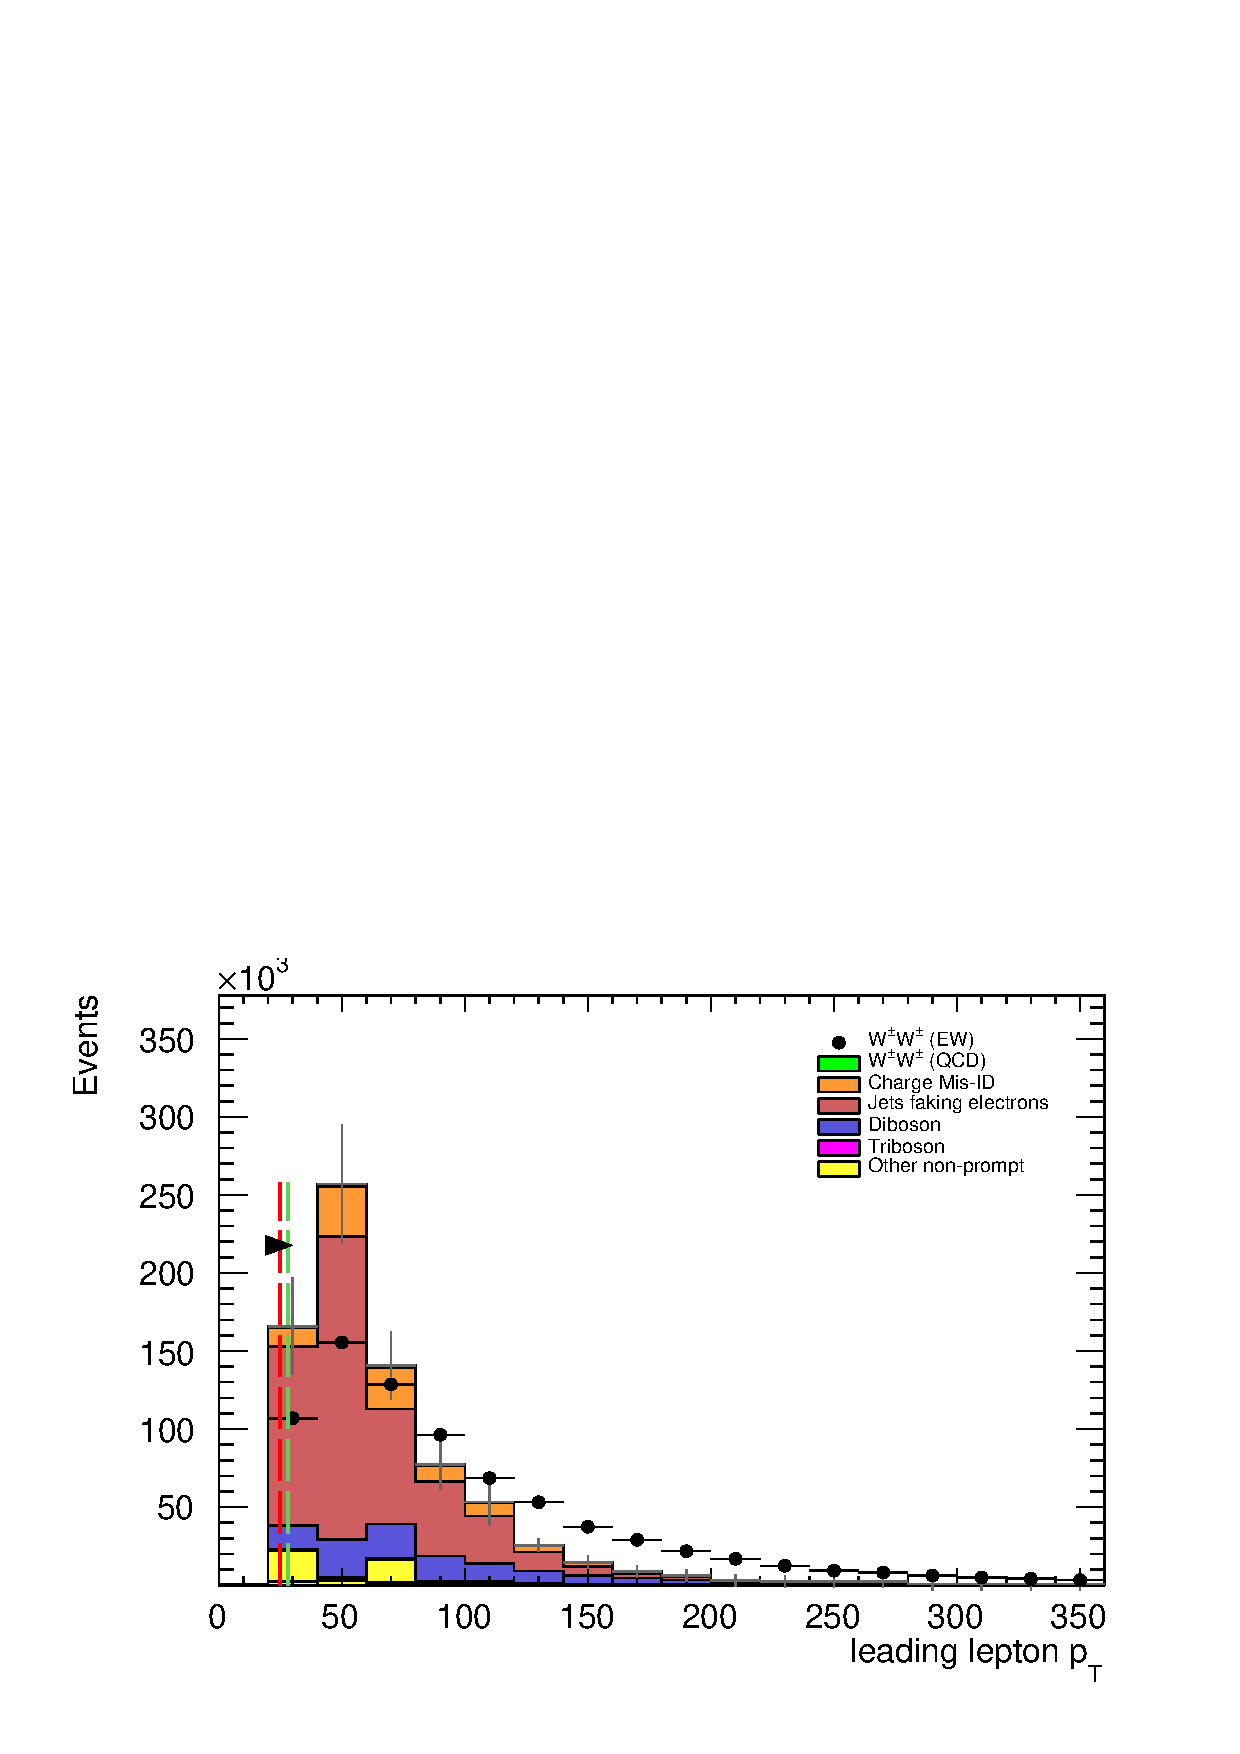
\includegraphics[width=0.6\textwidth]{figs/ssww_upgrade/optimization_plots/lep0pt}
  \caption{Leading lepton $\pt$ distribution.  The default and optimized cuts are represented by the red and green dashed lines, respectively.  The \ssww EWK signal (black points) is normalized to the same area as the sum of the backgrounds (colored histogram).}
  \label{fig:optimized_lep0pt}
\end{figure}

\begin{figure}[htp]
  \centering
  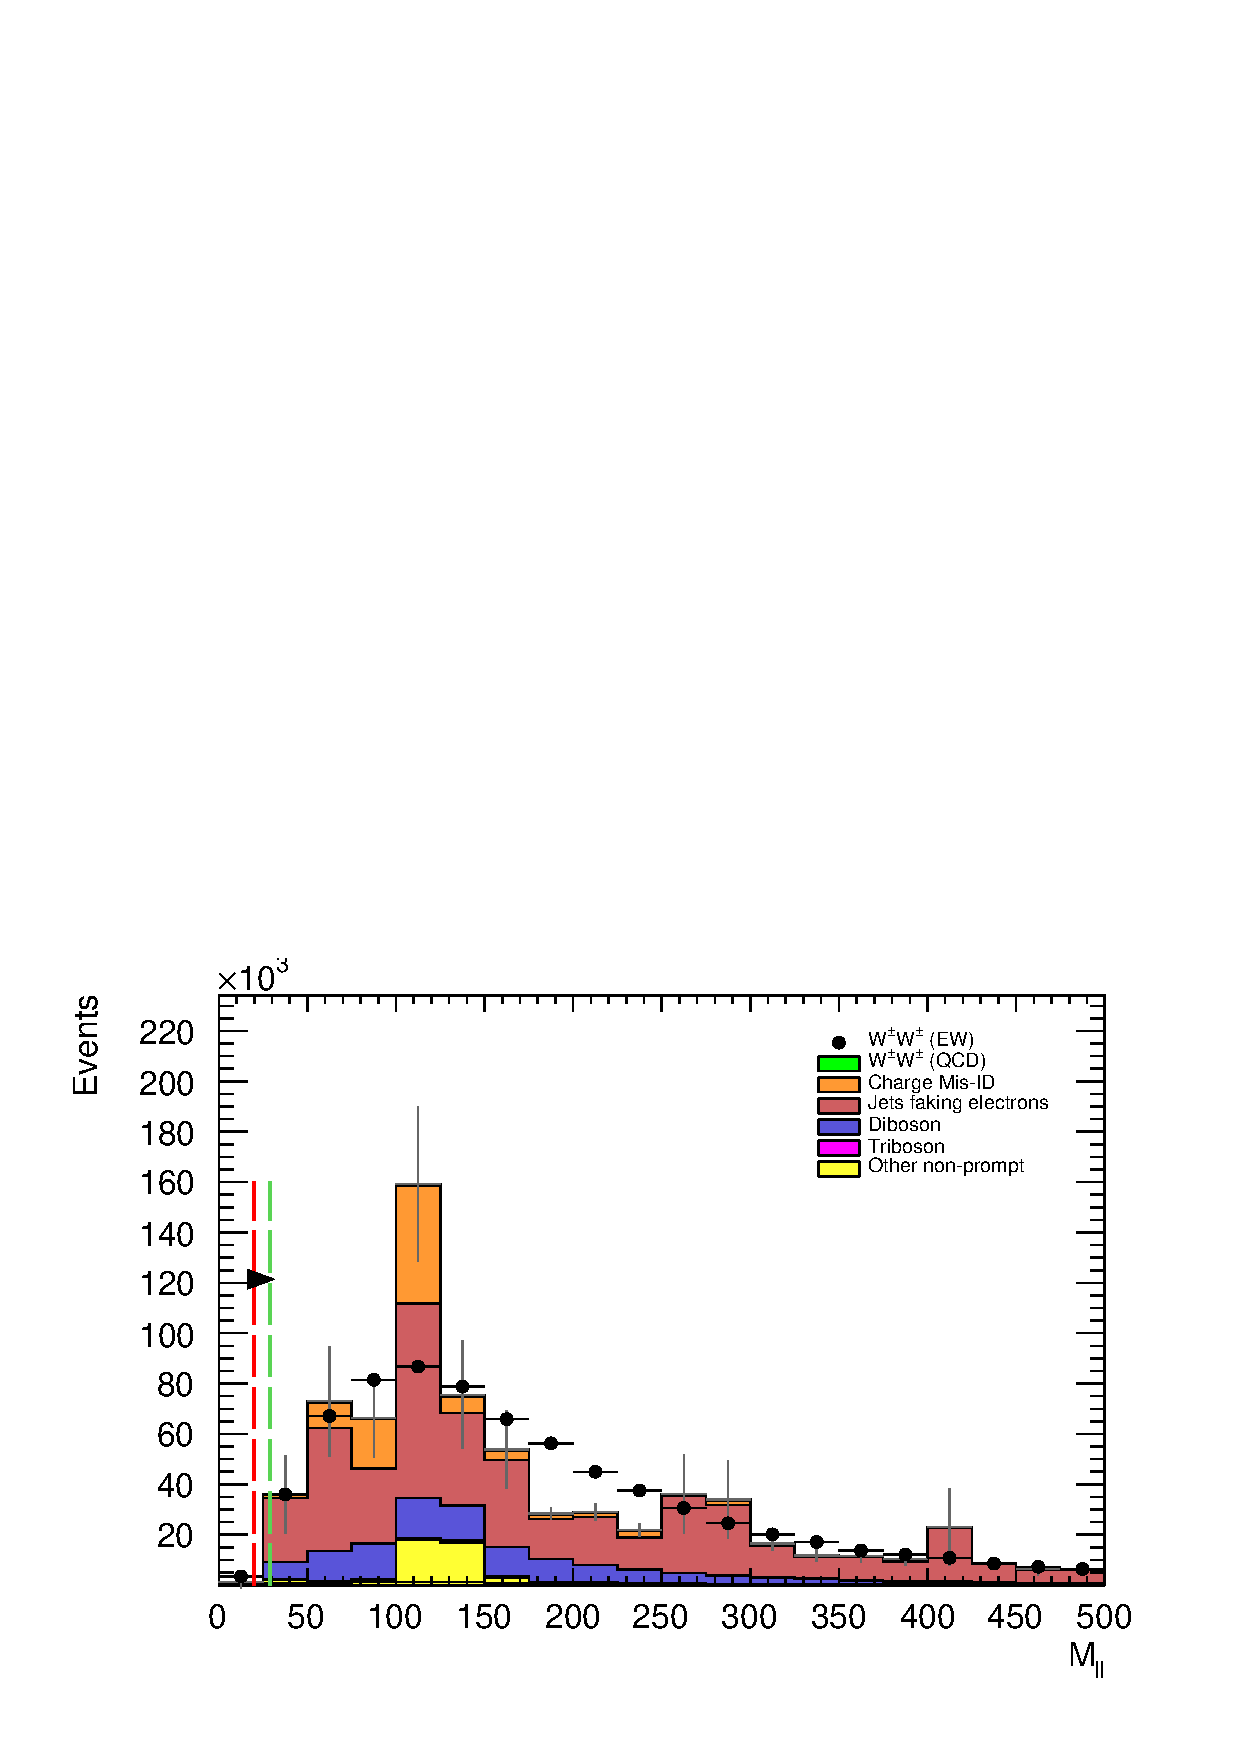
\includegraphics[width=0.6\textwidth]{figs/ssww_upgrade/optimization_plots/mll}
  \caption{Dilepton invariant mass distribution.  The default and optimized cuts are represented by the red and green dashed lines, respectively.  The \ssww EWK signal (black points) is normalized to the same area as the sum of the backgrounds (colored histogram).}
  \label{fig:optimized_mll}
\end{figure}

\begin{figure}[htp]
  \centering
  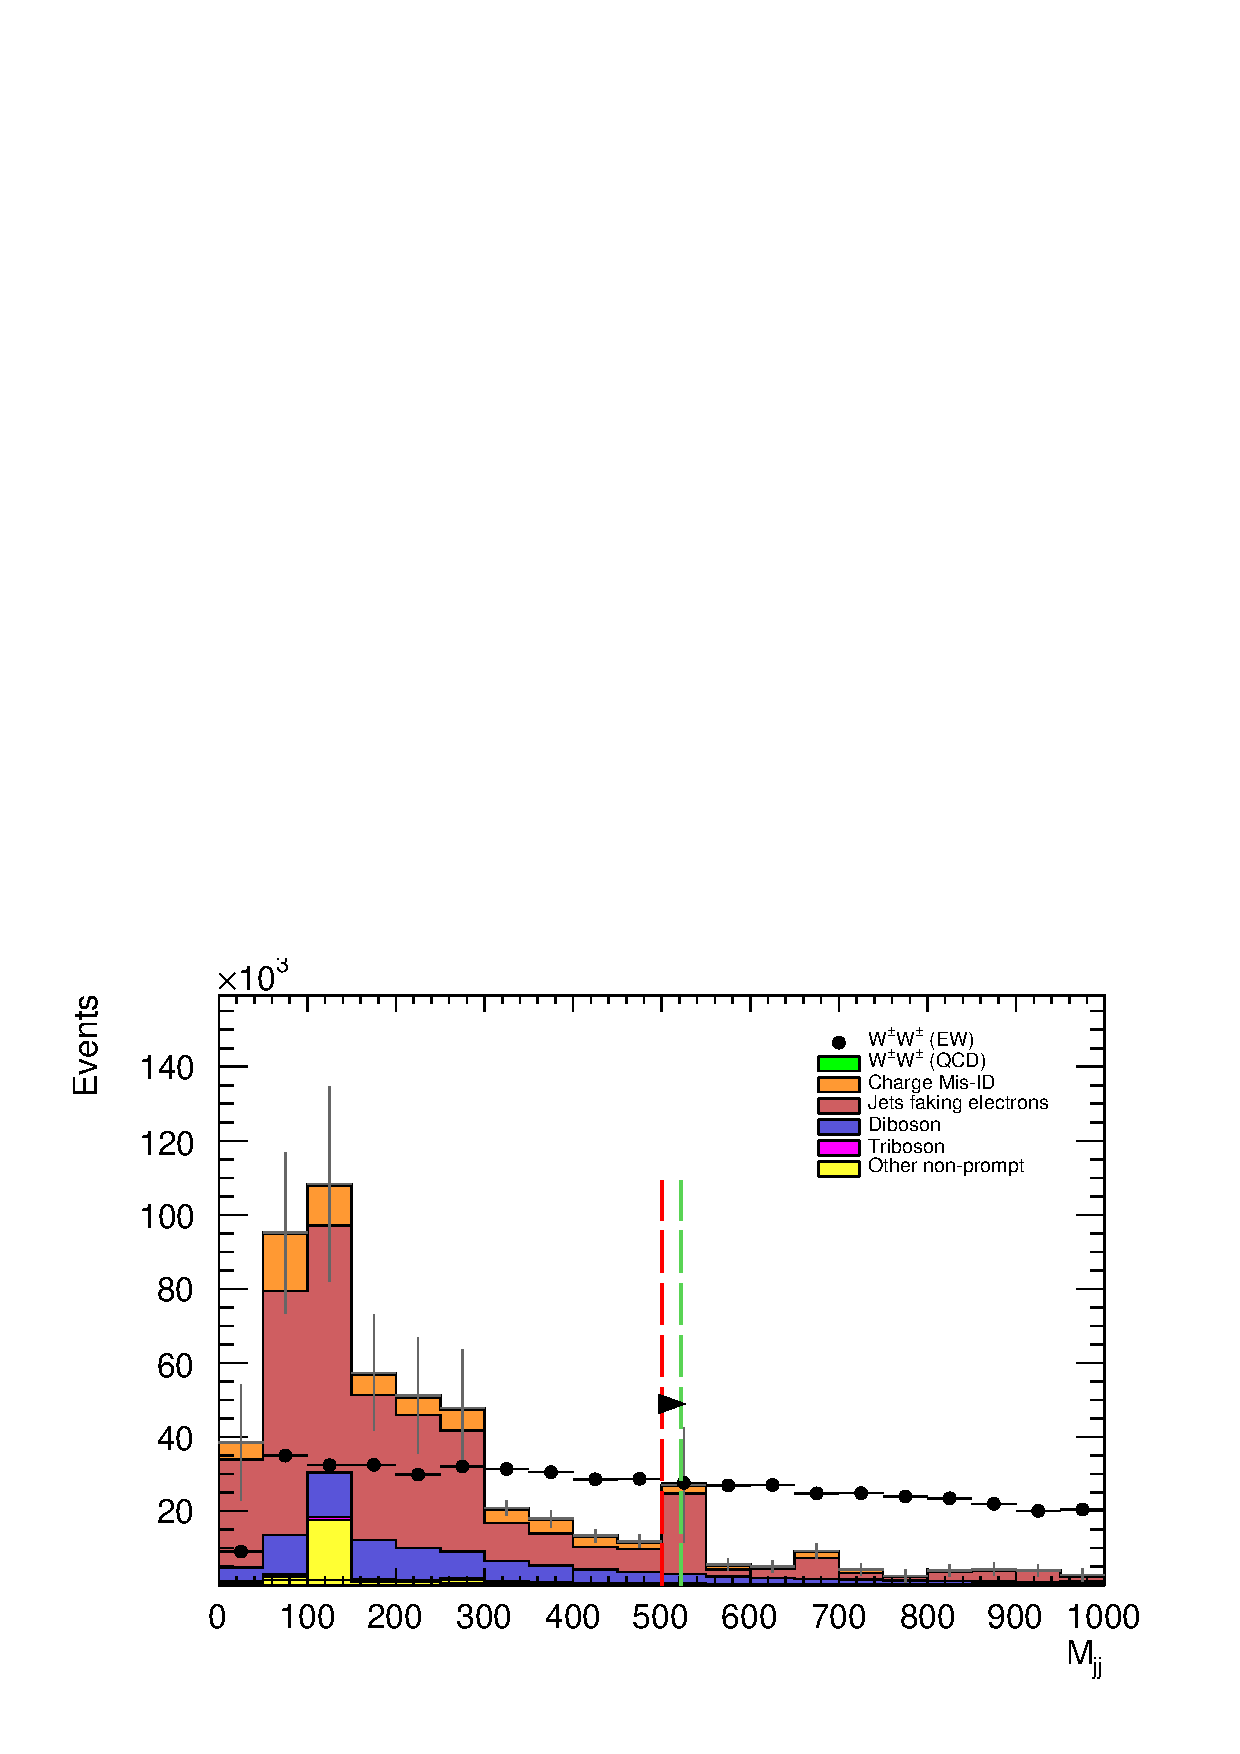
\includegraphics[width=0.6\textwidth]{figs/ssww_upgrade/optimization_plots/mjj}
  \caption{Dijet invariant mass distribution.  The default and optimized cuts are represented by the red and green dashed lines, respectively.  The \ssww EWK signal (black points) is normalized to the same area as the sum of the backgrounds (colored histogram).}
  \label{fig:optimized_mjj}
\end{figure}
\FloatBarrier

